\documentclass[12pt]{article}
\setlength{\oddsidemargin}{0in}
\setlength{\evensidemargin}{0in}
\setlength{\textwidth}{6.5in}
\setlength{\parindent}{0in}
\setlength{\parskip}{\baselineskip}

\usepackage{colortbl}
\usepackage{xcolor}
\usepackage{amsmath,amsfonts,amssymb}
\usepackage{qtree}
\usepackage{enumerate}
\usepackage{multirow}
\usepackage{graphicx}
\usepackage{forest}
\usepackage{tabularx}
\usepackage{pbox}

\begin{document}
CSCI 4448 Spring 2017 \hfill Project Write-up 2\\
\textbf{Project: } Cheap Chef \\
\textbf{Name: } Ethan Wright \\


\hrulefill
%%%%%%%%%%%%%%%%%%%%%%%%% SECTION 1  %%%%%%%%%%%%%%%%%%%%%%%%%
\begin{center}
  \textbf{Use Case Document}
  \begin{tabular}{l  l}
    \textbf{User ID} & \textbf{Requirement} \\ \hline \rowcolor[gray]{.95}
    UR-001 & The user can select an ingredient from a category \\
    UR-002 & The user can select an ingredient from a search function \\ 
  \end{tabular}
\end{center}
\newpage
\begin{center}
  \textbf{Use Cases}
\end{center}
\textbf{Requirements: } \\
\textbf{UR-001: } As a user I want to be able to select my ingredient out of a category \\
\textbf{UR-002: } As a user I want to be able to search for my ingredient \\ 
\vspace{1cm}

\textbf{Use Case Documents:} \\
  \begin{tabular}{ l | l }
    \hline
    \textbf{Use Cases} & UR-001 \\ \rowcolor[gray]{.95}
    \textbf{Use Case Name} & As a user, I can choose an ingredient from a category \\ 
    \textbf{Description} & User has option to display categories of ingredients \\ \rowcolor[gray]{.95}
    \textbf{Actors} & User \\
    \textbf{Pre-conditions} & None \\ \rowcolor[gray]{.95}
    \textbf{Post-conditions} & Ingredients in category displayed to user \\ 
    \textbf{Frequency of Use} & When ever user wants to choose ingredient but not search for it \\ \rowcolor[gray]{.95}
    \textbf{Flow of Events} & \pbox{20cm}{\textbf{Actor Action: } Click on desired category\\ \textbf{System Response:} Return
    all ingredients matching category} \\ 
    \textbf{Variations} & User does not select ingredient \\  \rowcolor[gray]{.95}
    \textbf{Exceptions} & If too many ingredients exist it shouldn't allow an addition \\
    \textbf{Developer Notes} & Depicted in Figure \ref{fig:UR-001} \\ \hline
  \end{tabular}


  \begin{tabular}{ l | l }
    \hline
    \textbf{Use Cases} & UR-002 \\ \rowcolor[gray]{.95}
    \textbf{Use Case Name} & As A user, I can search for an ingrediente to add  \\ 
    \textbf{Description} & User can enter text into search bar to display results \\ \rowcolor[gray]{.95}
    \textbf{Actors} & User \\
    \textbf{Pre-conditions} & None \\ \rowcolor[gray]{.95}
    \textbf{Post-conditions} & User has list of ingredients to select from \\ 
    \textbf{Frequency of Use} & When the user wants to choose an ingredient but not just use a category \\ \rowcolor[gray]{.95}
    \textbf{Flow of Events} & \pbox{20cm}{\textbf{Actor Action: }Enter an ingredient into the search bar \\
    \textbf{System Repsonse:} Return a list of all matching ingredients }  \\
    \textbf{Variations} & No matching ingredients are found \\  \rowcolor[gray]{.95}
    \textbf{Exceptions} & If no ingredient is found it should recommend a similar ingredient \\
    \textbf{Developer Notes} &  Depicted in Figure \ref{fig:UR-002}\\ \hline
  \end{tabular}
 
 \newpage
 \begin{figure}
   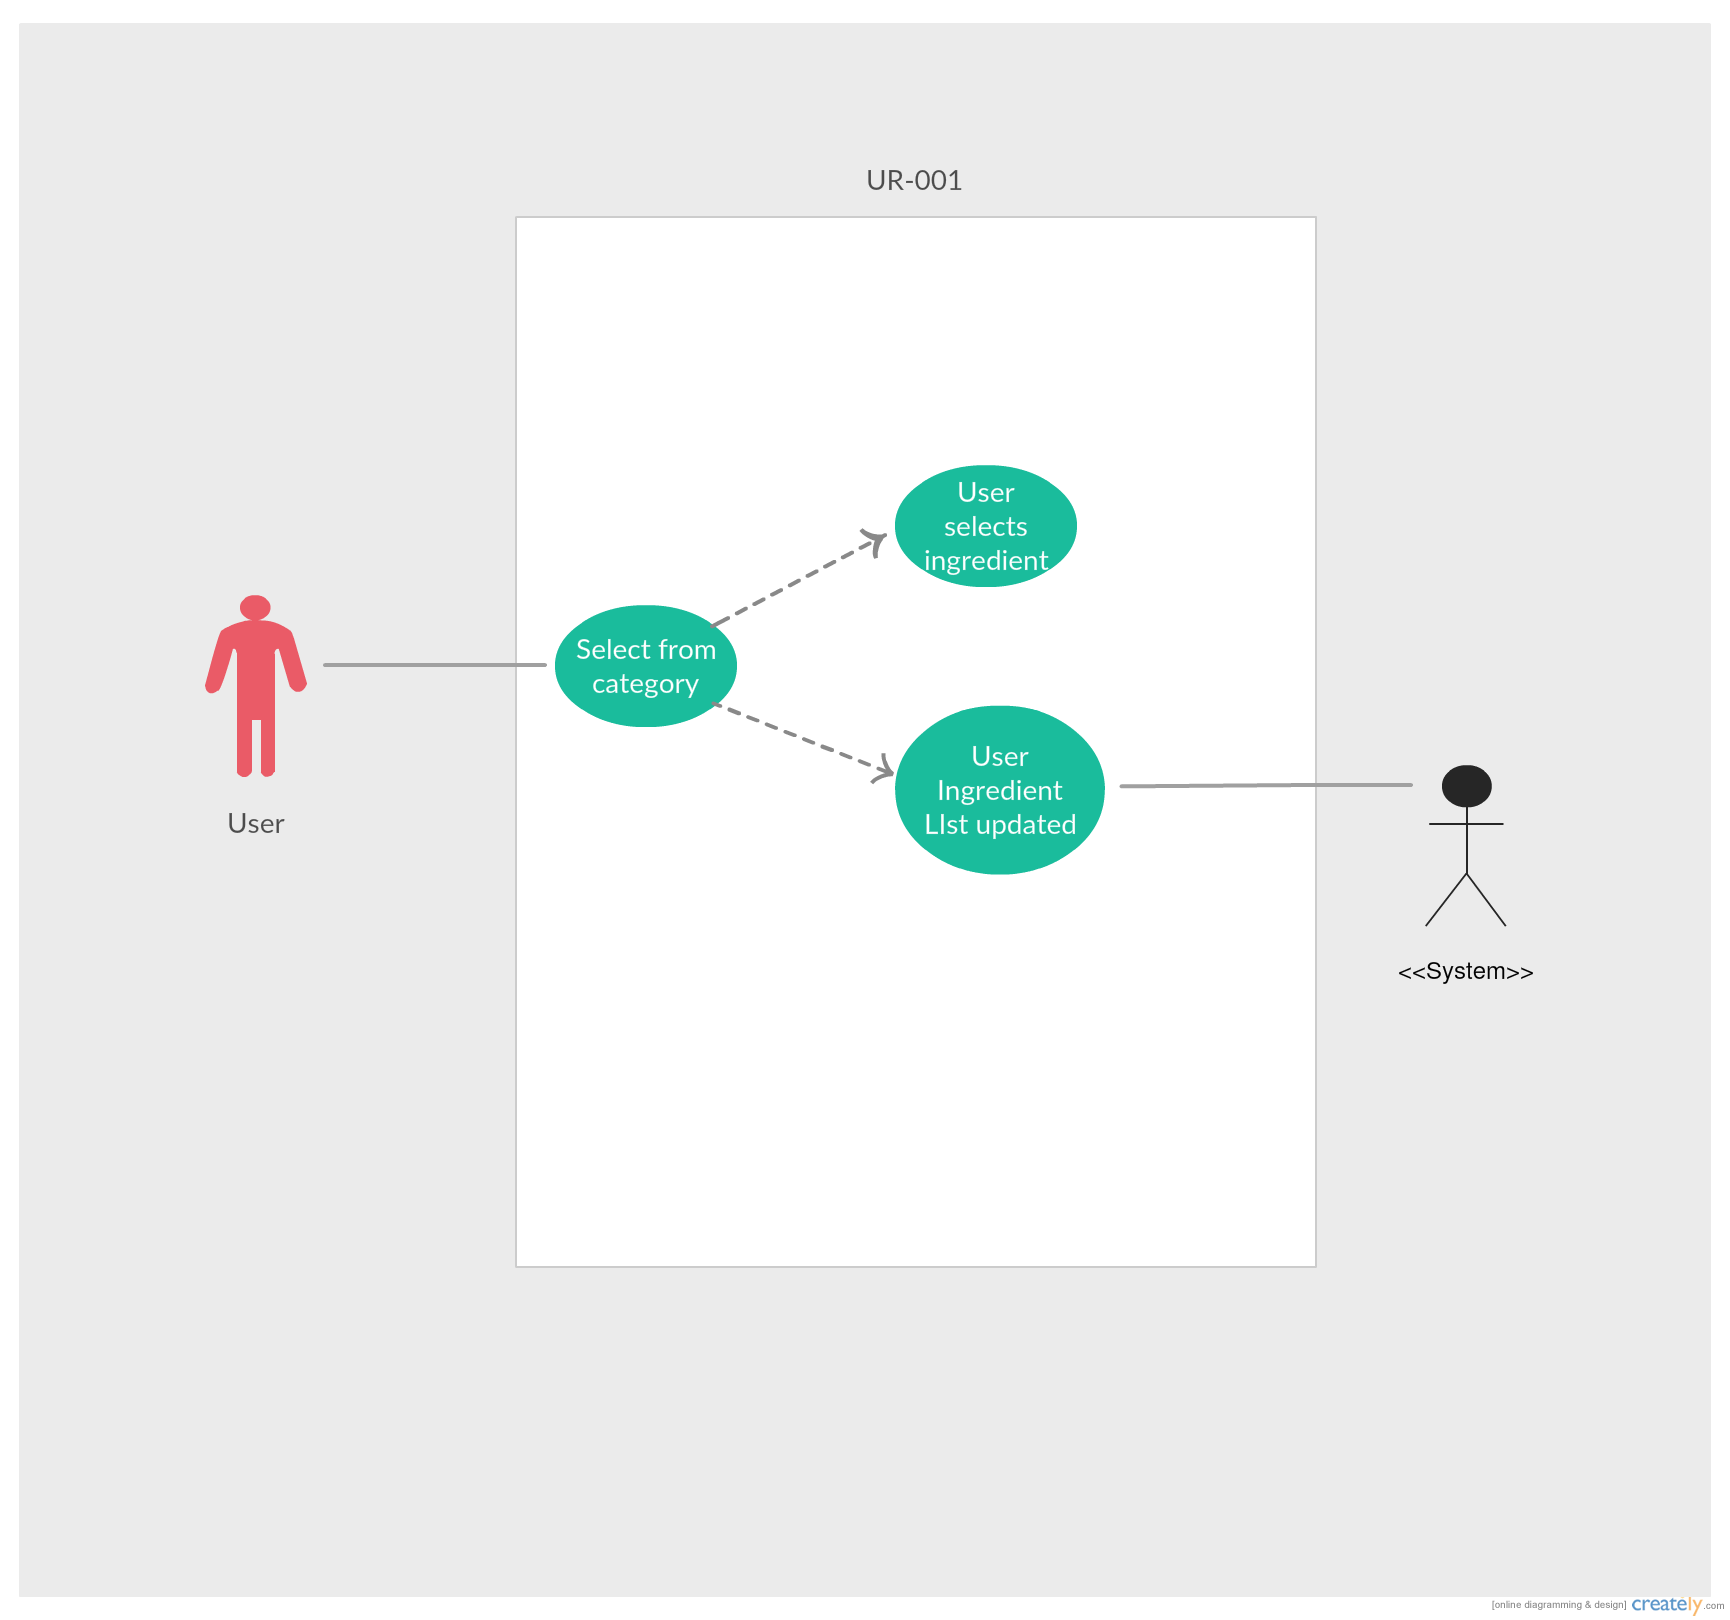
\includegraphics[width=\linewidth]{UR-001.png}
   \caption{UR-001}
   \label{fig:UR-001}
 \end{figure}
 \newpage
 \begin{figure}
   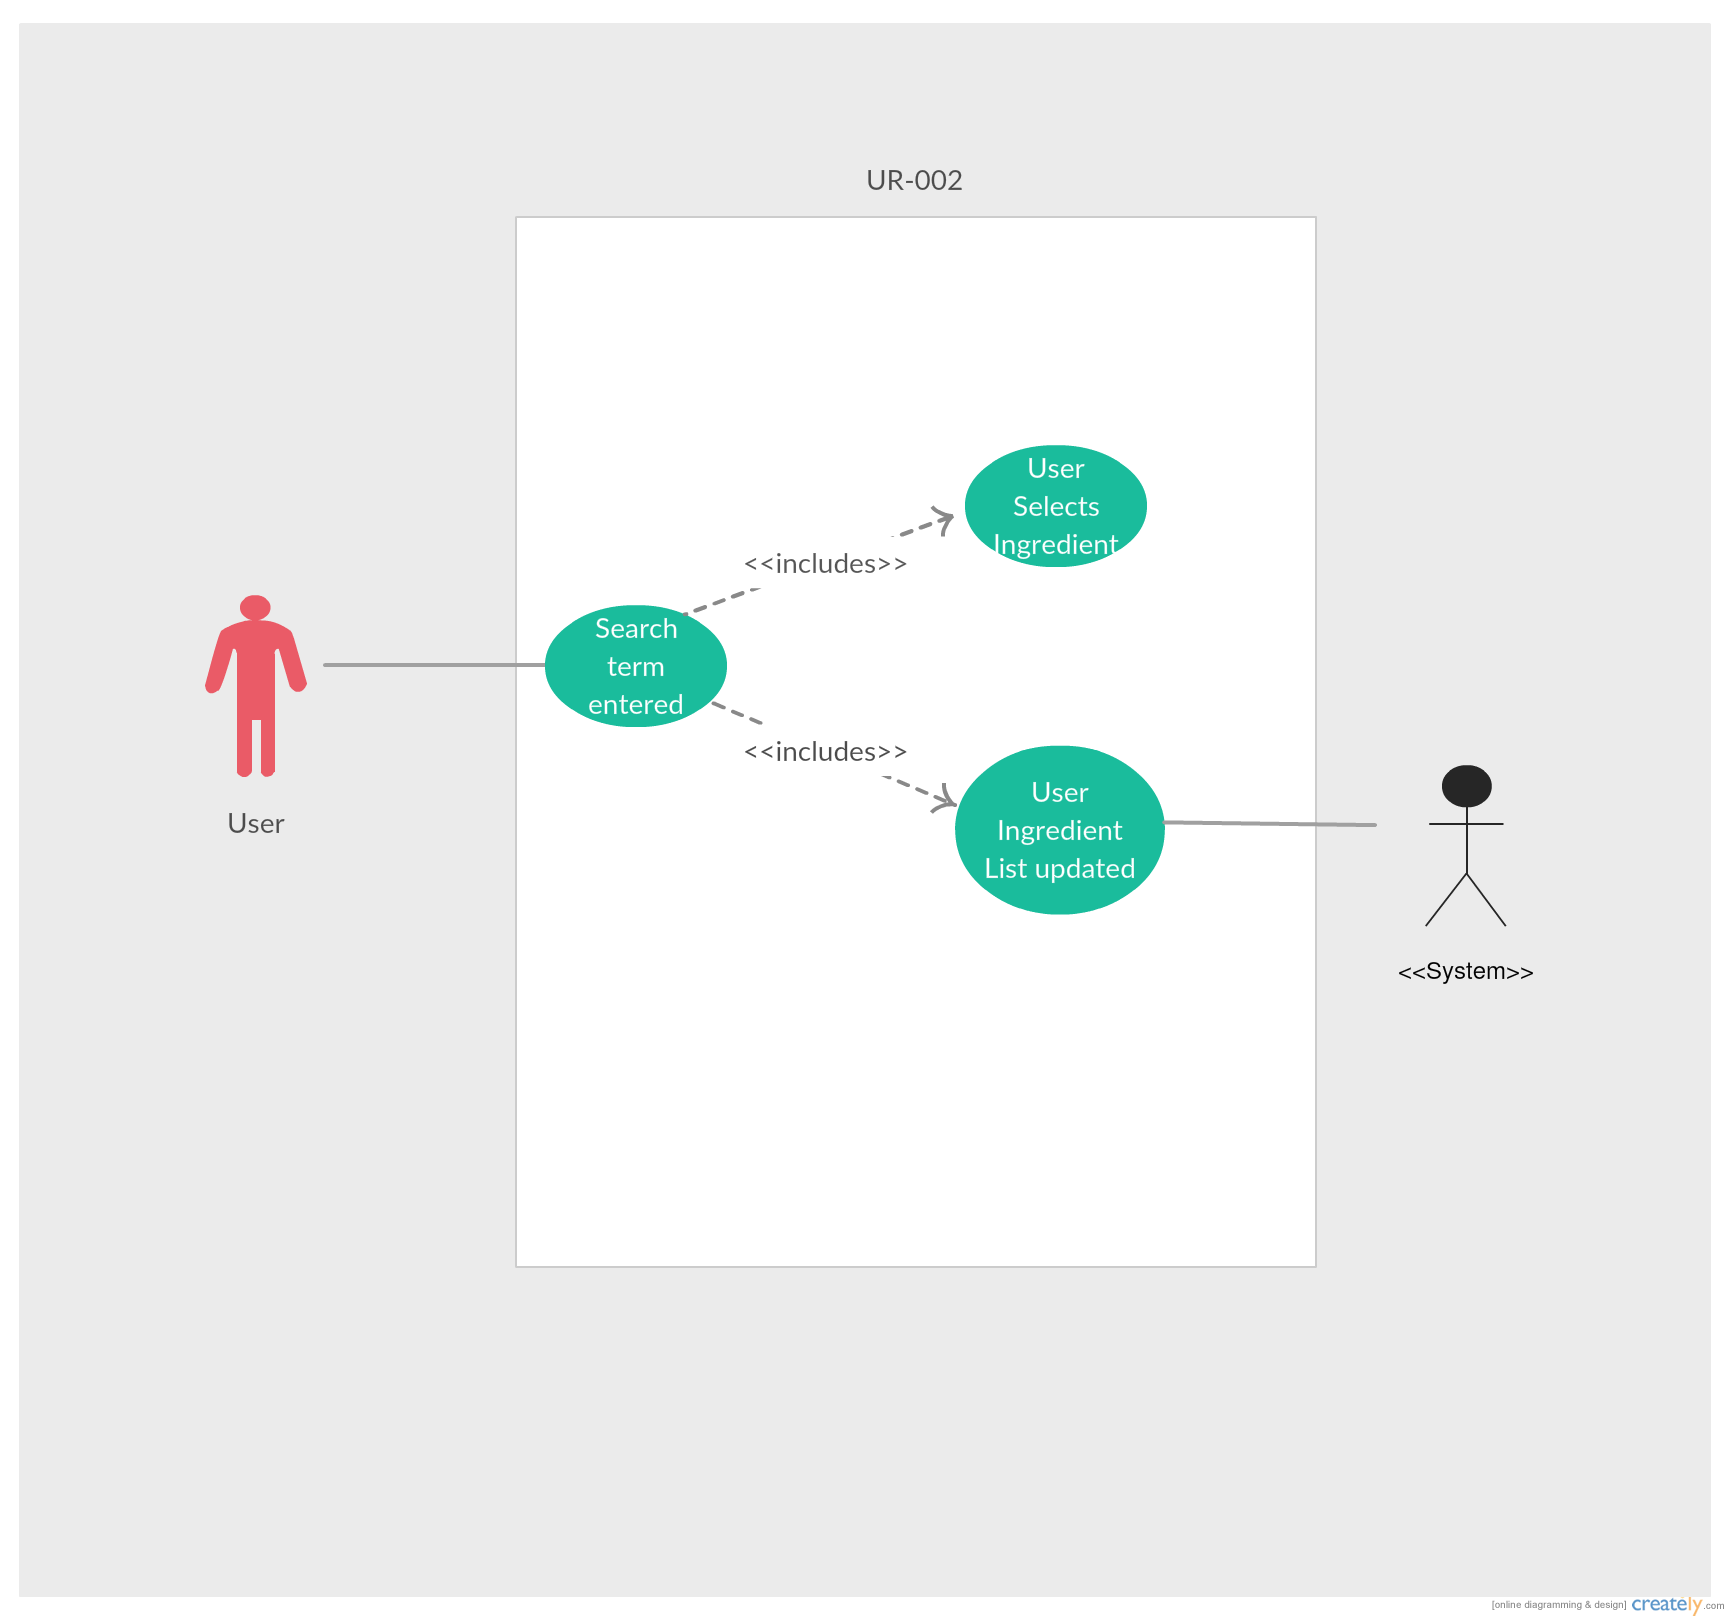
\includegraphics[width=\linewidth]{UR-002.png}
   \caption{UR-002}
   \label{fig:UR-002}
 \end{figure}
 \newpage

\begin{figure}
  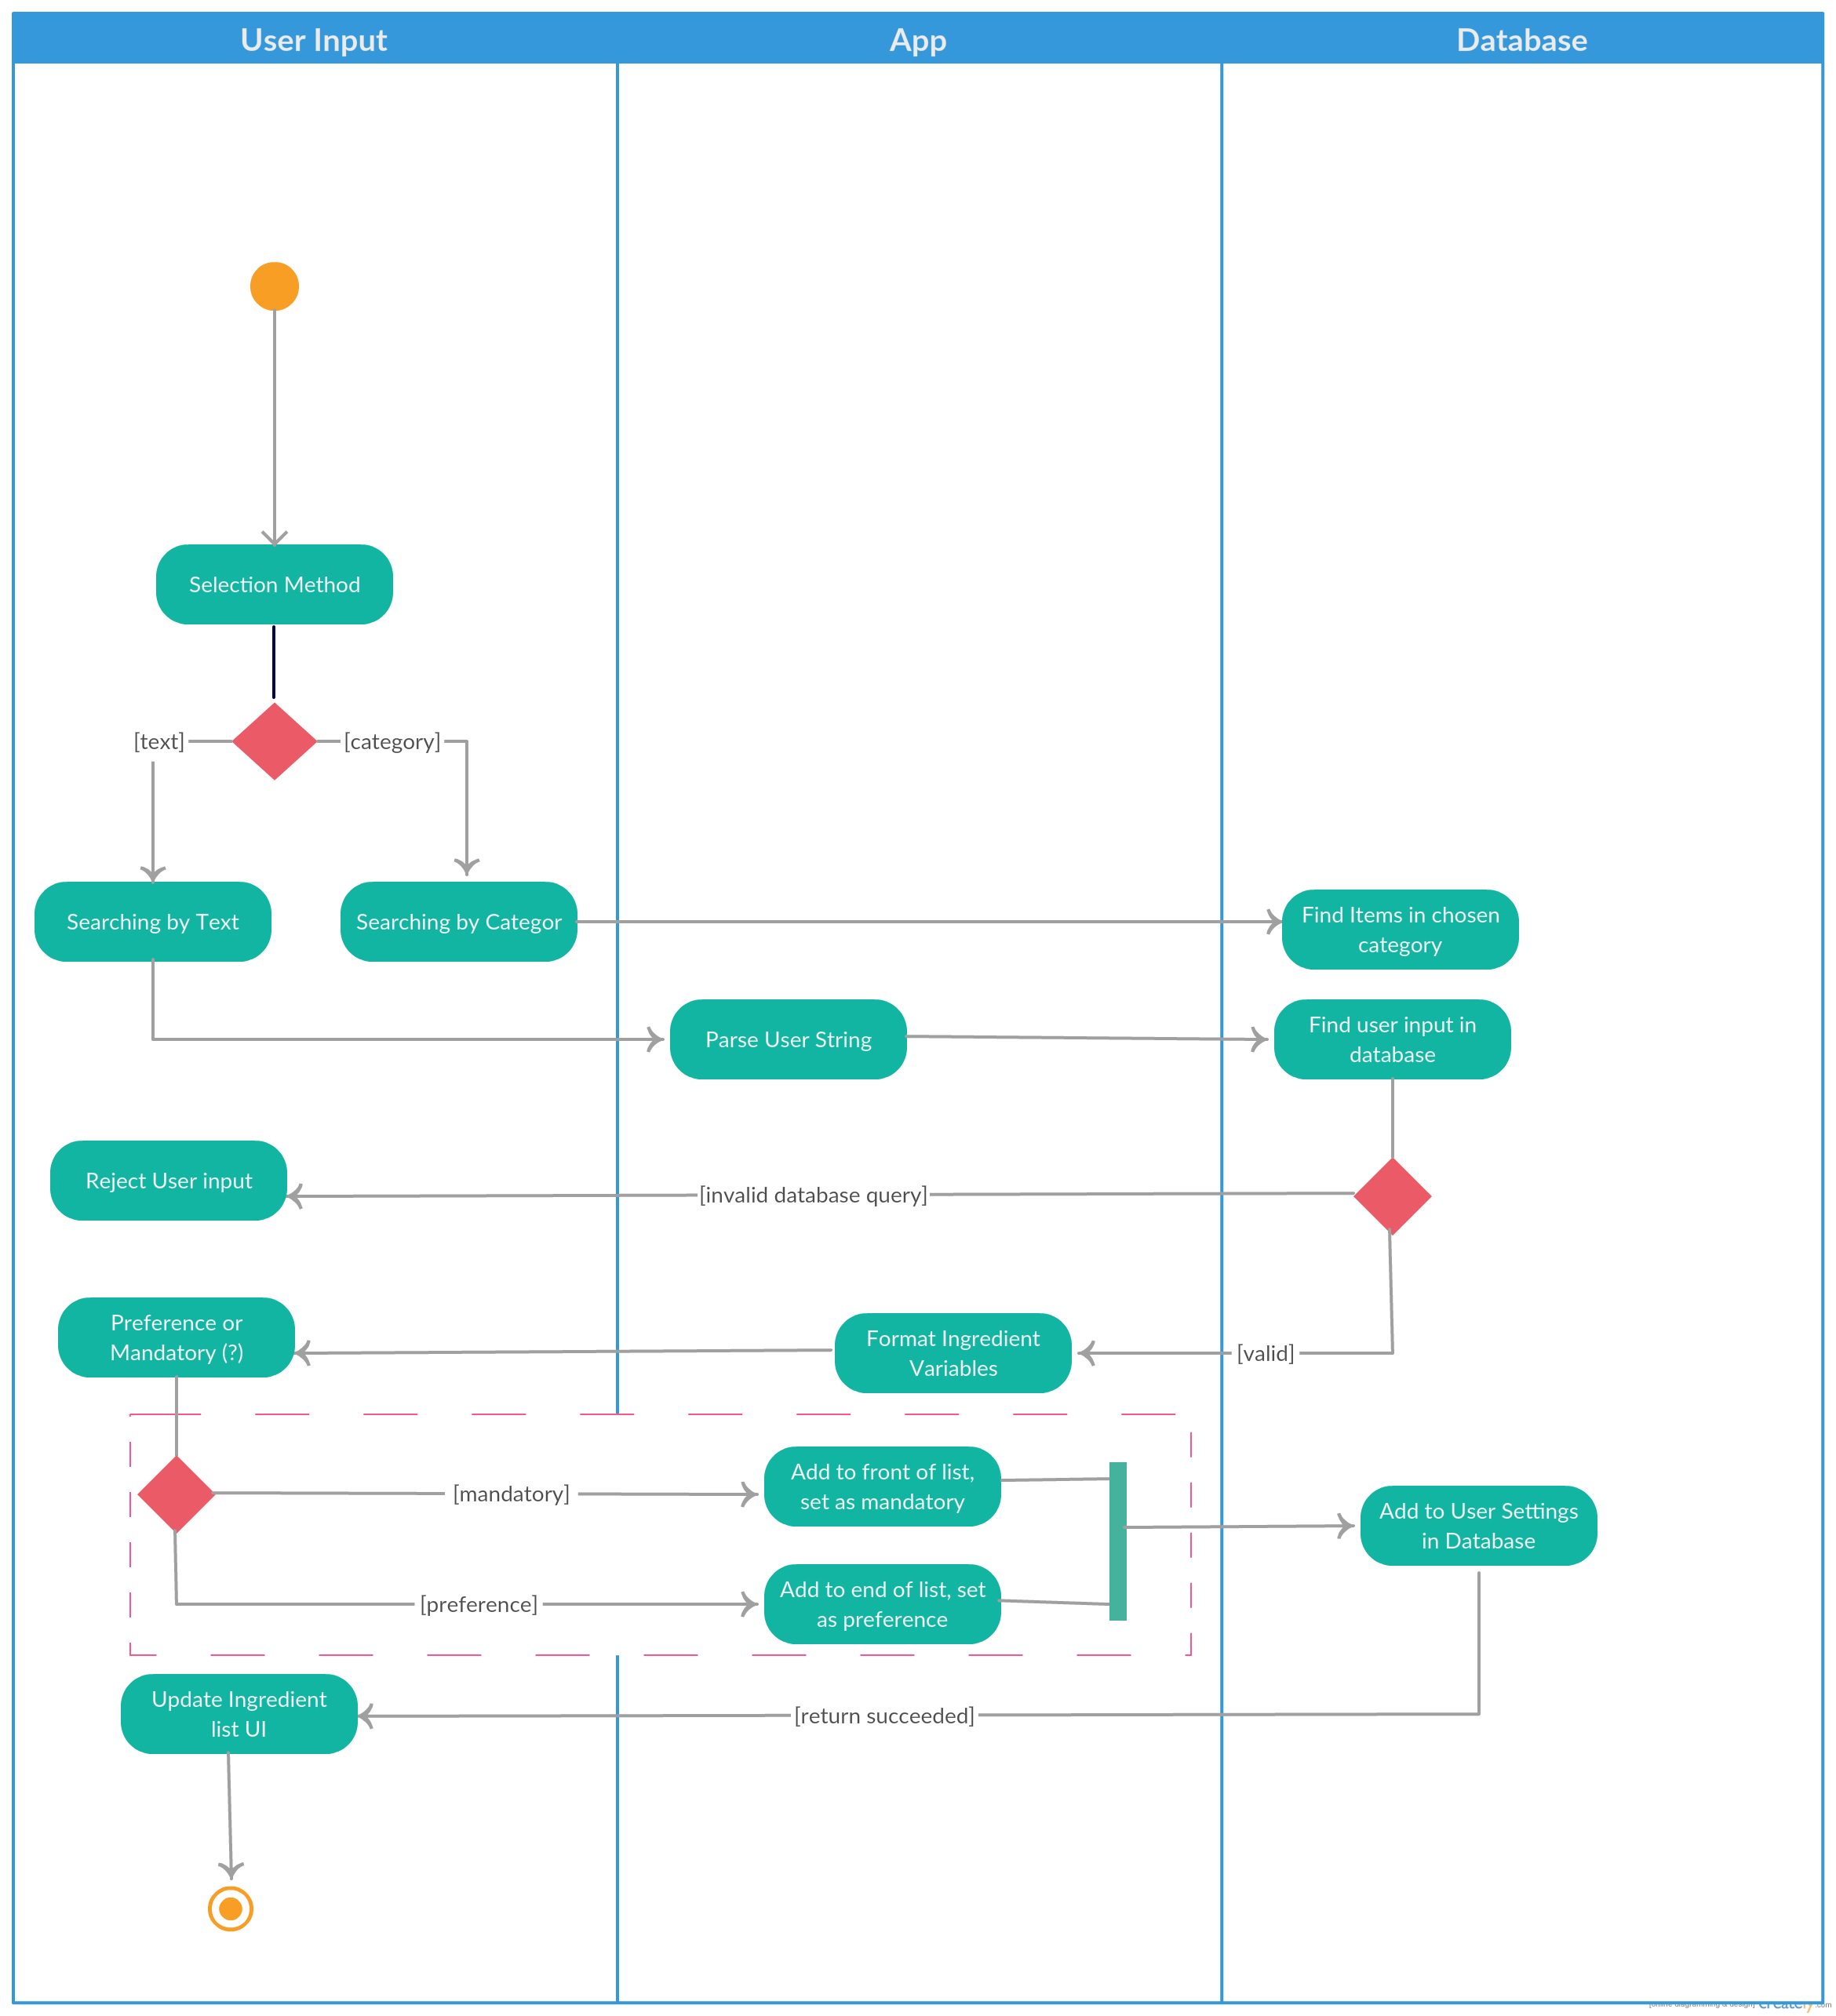
\includegraphics[width=\linewidth]{activity.png}
  \caption{Activity Diagram}
  \label{fig:activity}
\end{figure}

\newpage
\begin{figure}
    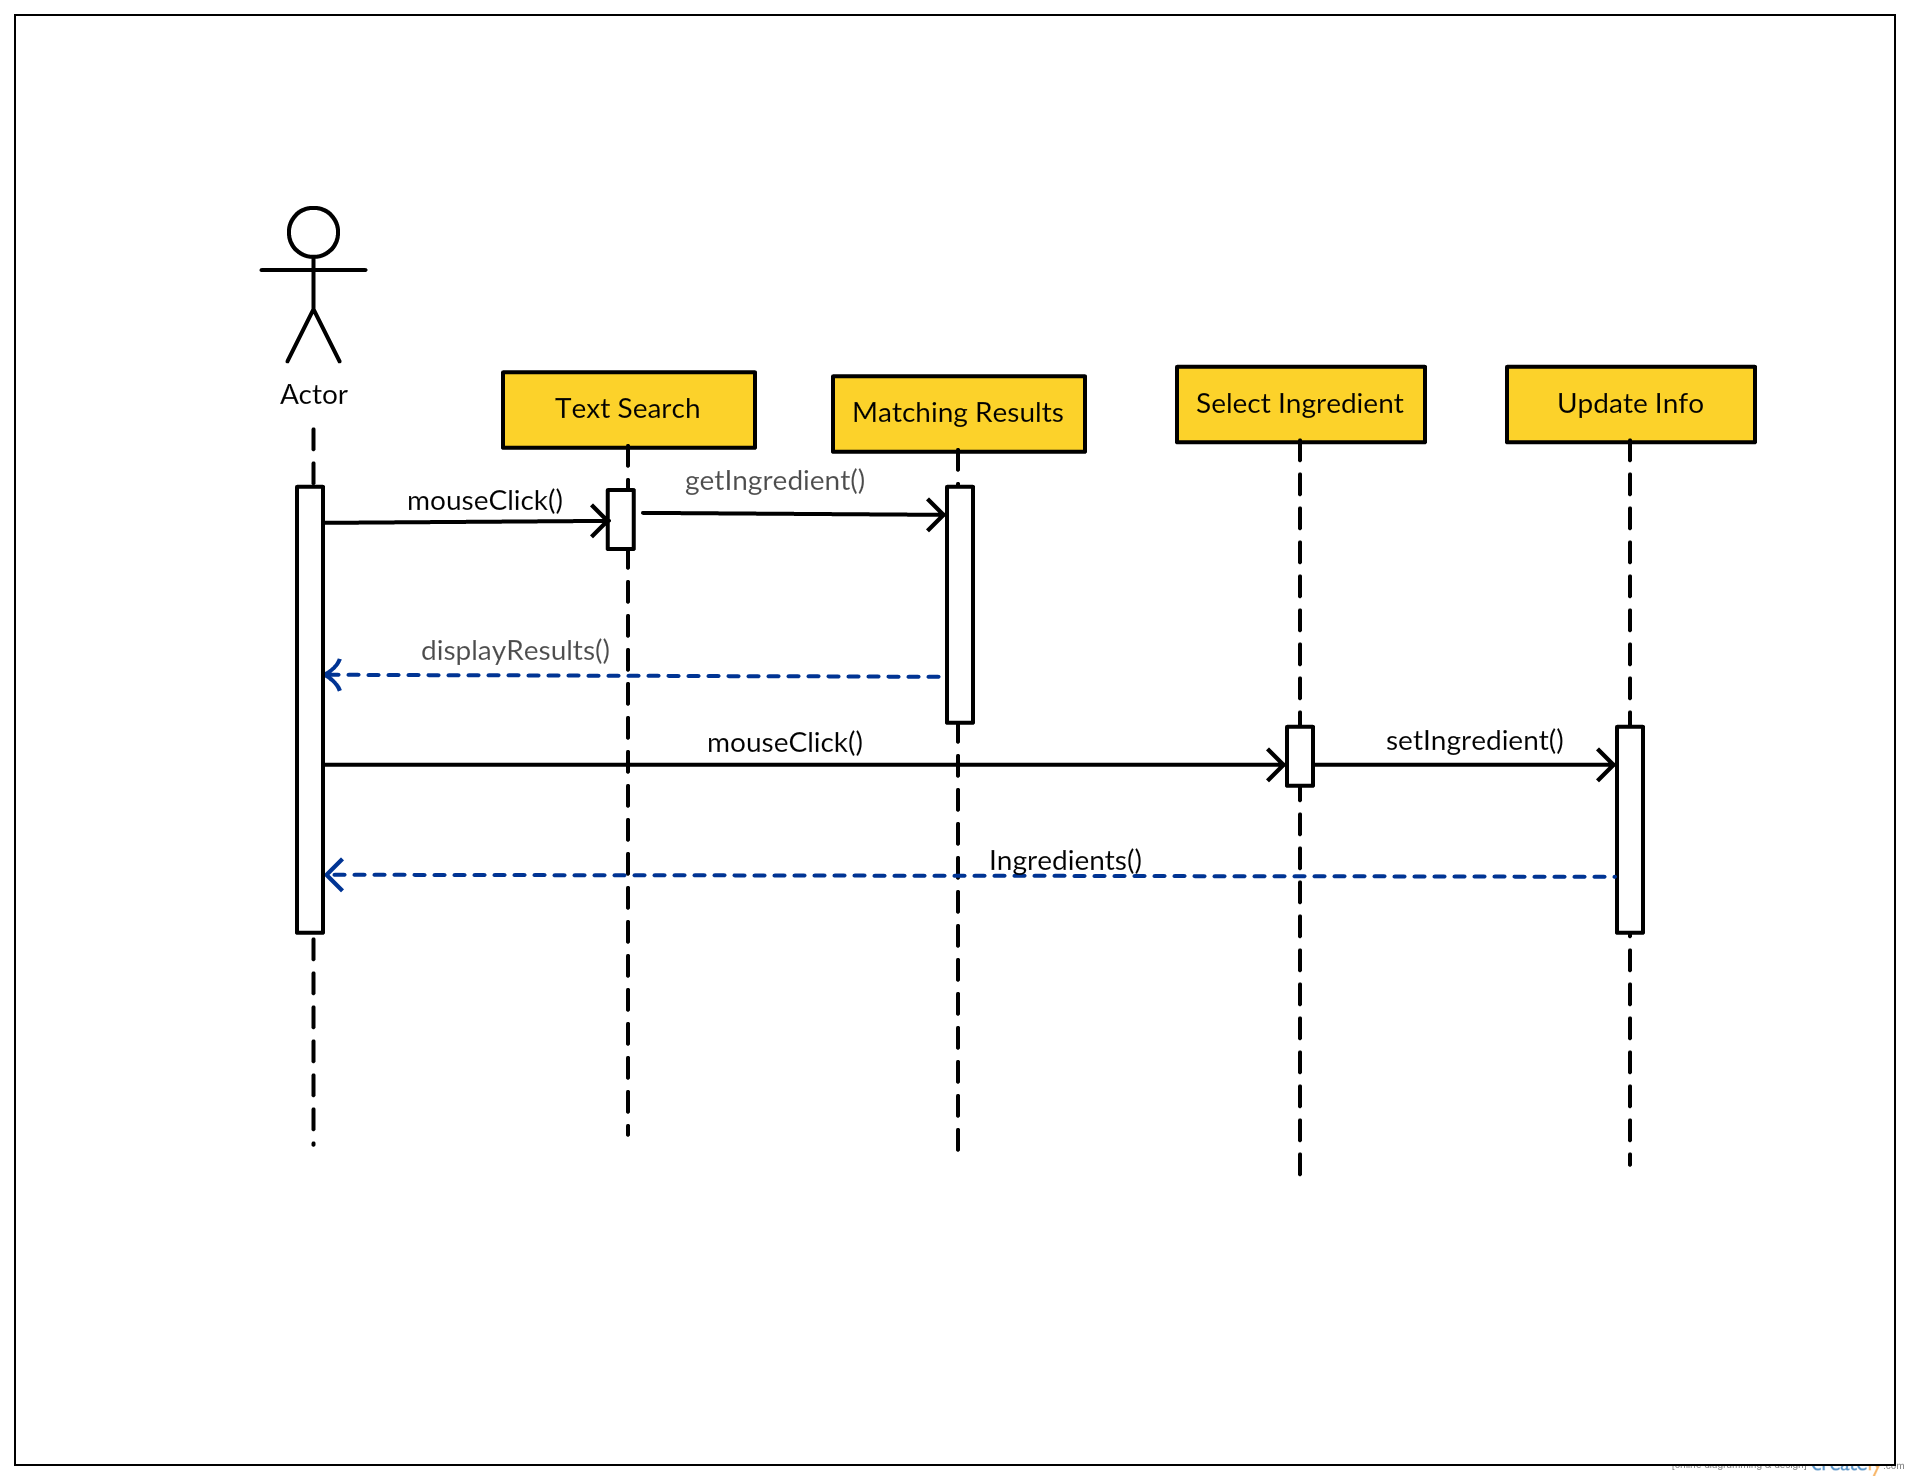
\includegraphics[width=\linewidth]{sequence.png}
    \caption{Sequence Diagram}
    \label{fig:sequence}
\end{figure}
\end{document}
